%*******************************************************************************
%*******************************************************************************
\chapter{Songbook-Client}
\setcounter{chapter}{2}
\label{chap:songbook-client}
\minitoc
%*******************************************************************************
%*******************************************************************************

The \client{} application is a graphical interface to build customized
songbooks\footnote{\url{http://www.ohloh.net/p/songbook-client},
  \url{http://github.com/crep4ever/songbook-client}}.

\begin{nota}
Independently of your operating system, the songbook's dependencies must
have been installed first (mainly \LaTeX{} and Python) in order to
build a pdf songbook. See \refsec{sec:install} for instructions.
\end{nota}

Downloads are available at \url{http://www.patacrep.com/static1/downloads}


%*******************************************************************************
\section{Interface}
%*******************************************************************************

%-------------------------------------------------------------------------------
\subsection{First launch}
%-------------------------------------------------------------------------------

\begin{figure}
  \centering
  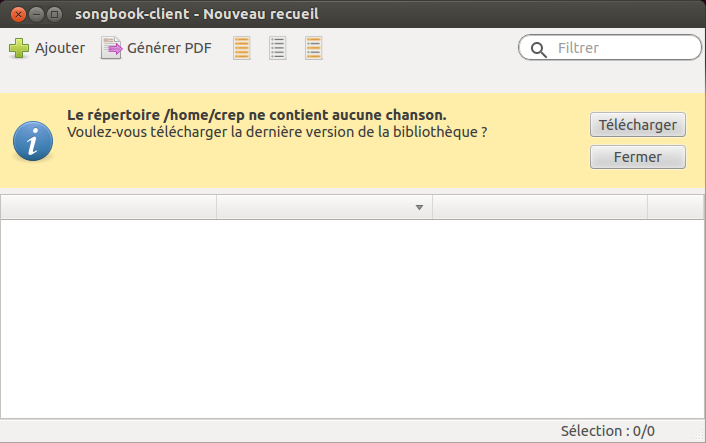
\includegraphics[width=\textwidth]{start}
  \caption{First launch of the application.}
  \label{fig:start}
\end{figure}

By default, the interface presents an empty list
(\reffig{fig:start}). The \client{} must be linked to an existing
\recueil{}. There are two options:

\begin{enumerate}
\item Indicate the path of a \directory{songbook} directory that is on
  your hard drive from the menu \menu{Edition}{Preferences}
  (\reffig{fig:solution-a}).
\item Download the latest version from the Internet from the menu
  \menu{Library}{Download} (\reffig{fig:solution-b}).
\end{enumerate}

Once the \client{} is linked to a \recueil{}, the \emph{songs'
  library} is built from the \ext{sg} files that have been found in
the \directory{songs} sub-directory of the \recueil{}.


%%%%%%%%%%%%%%%%%%%%%%%%%%%%%% FIGURE %%%%%%%%%%%%%%%%%%%%%%%%%%%%%%%%%%
\begin{figure}
  \centering
  %% -- subfigures --
  \subfigure[]{
    \label{fig:solution-a}
    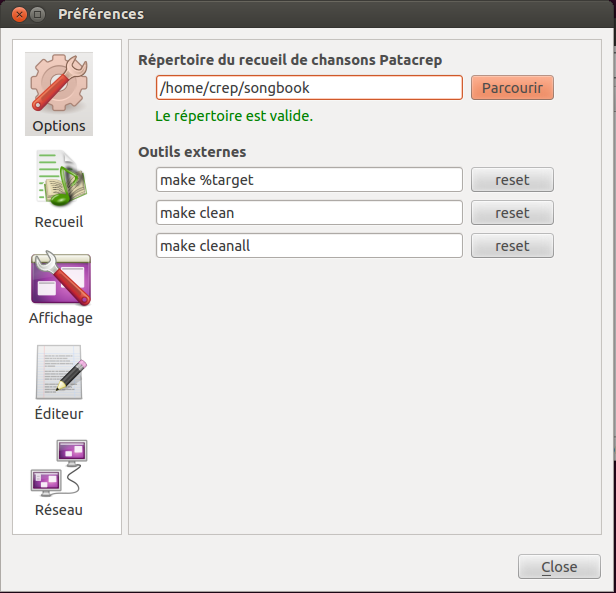
\includegraphics[width=0.45\textwidth]{preferences}%
  }%
  \hspace{0.1cm}%
  \subfigure[]{%
    \label{fig:solution-b}%
    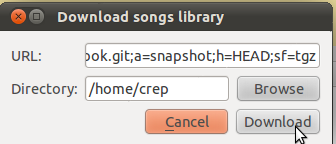
\includegraphics[width=0.45\textwidth]{download}%
  }%
  %% -- subfigures --
  \caption{% 
    Two options allow to link the \emph{Songbook-Client} to a \recueil{}.
    \subref{fig:solution-a}~Indicate the path to a songbook directory;%
    \subref{fig:solution-b}~Download from the Internet.%
  }%
  \label{fig:solutions}
\end{figure}
%%%%%%%%%%%%%%%%%%%%%%%%%%%%%%%%%%%%%%%%%%%%%%%%%%%%%%%%%%%%%%%%%%%%%%%%


%-------------------------------------------------------------------------------
\subsection{The songs' library}
%-------------------------------------------------------------------------------

\begin{figure}
  \centering
  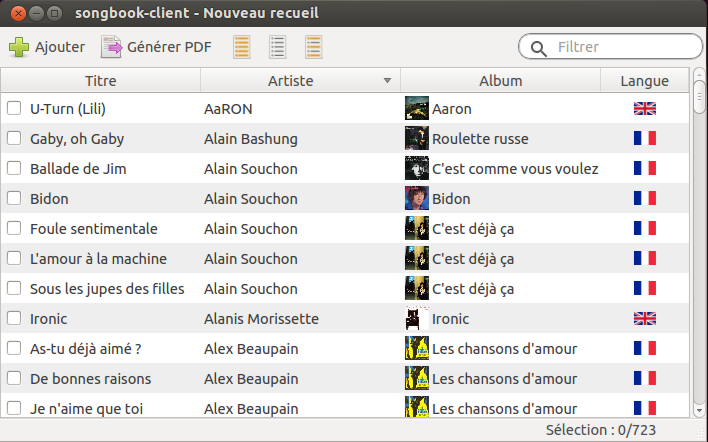
\includegraphics[width=.7\textwidth]{library}
  \caption{The songs' library.}
  \label{fig:library}
\end{figure}

The set of \ext{sg} songs found in the \directory{songs} sub-directory
is displayed as a list. Columns may be hidden/displayed in the tab
\command{Display} from the menu \menu{Edition}{Preferences}. By
default, the only visible columns are \command{Title}, \command{Artist} and
\command{Album}.

The songs in the library can be selected with a simple click.  A
selected song is highlighted. Click on a selected song to deselect it.

%*******************************************************************************
\section{Adding a new song}
%*******************************************************************************

The menu \menu{Library}{New song} allows to add a new song to the
library (\reffig{fig:new-song-a}). The dialog allows to set song's
meta-data such as its title, author etc. These fields allow to
generate the skeleton of the new file \ext{sg} corresponding to the
song (\reffig{fig:new-song-b}). The third step
(\reffig{fig:new-song-c}) consists in writing the guitar tab. Finally,
the song can be selected in the library to obtain the pdf from the
menu \menu{Songbook}{Build PDF} (\reffig{fig:new-song-d}).

%%%%%%%%%%%%%%%%%%%%%%%%%%%%%% FIGURE %%%%%%%%%%%%%%%%%%%%%%%%%%%%%%%%%%
\begin{figure}
  \centering
  %% -- subfigures --
  \subfigure[]{
    \label{fig:new-song-a}
    \includegraphics[width=0.35\textwidth]{new-song}%
  }%
  \hspace{0.1cm}%
  \subfigure[]{%
    \label{fig:new-song-b}%
    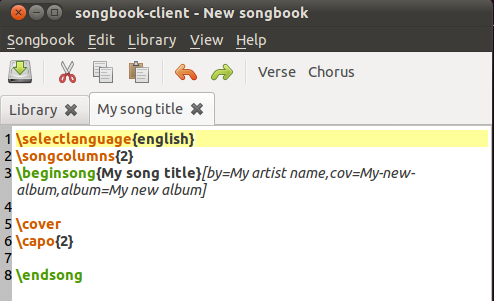
\includegraphics[width=0.6\textwidth]{song-editor-1}%
  }%
  \hspace{0.1cm}%
  \subfigure[]{%
    \label{fig:new-song-c}%
    \includegraphics[width=0.6\textwidth]{song-editor-2}%
  }%
  \hspace{0.1cm}%
  \subfigure[]{%
    \label{fig:new-song-d}%
    \includegraphics[width=0.35\textwidth]{result}%
  }%
  %% -- subfigures --
  \caption{%
    Add a new song.
    \subref{fig:new-song-a}~Meta-data information; %
    \subref{fig:new-song-b}~Auto generation of the \ext{sg} skeleton; %
    \subref{fig:new-song-c}~Write the guitar tab; %
    \subref{fig:new-song-d}~Build the pdf.%
  }%
  \label{fig:new-song}
\end{figure}
%%%%%%%%%%%%%%%%%%%%%%%%%%%%%%%%%%%%%%%%%%%%%%%%%%%%%%%%%%%%%%%%%%%%%%%%


%*******************************************************************************
\section{Making a customized songbook}
%*******************************************************************************

\paragraph{Save/Open}
The \ext{sb} file format saves the list of selected songs
and the options that define the appearance of a songbook
(see~\refsec{sec:create-songbook}).

\paragraph{Style and options of a songbook}
A dialog box allows to quickly select the main style (template) of the
songbook and its options (\reffig{fig:new-songbook}).

\begin{figure}
  \centering
  \includegraphics[width=\textwidth]{new-songbook}
  \caption{Customizing a songbook.}
  \label{fig:new-songbook}
\end{figure}

%*******************************************************************************
\section{Compiling from sources}
%*******************************************************************************

%-------------------------------------------------------------------------------
\subsection{\linux}
%-------------------------------------------------------------------------------

\paragraph{Dependencies}

\begin{unix}
  sudo apt-get install build-essential cmake
  sudo apt-get install libarchive-dev libhunspell-dev
  sudo apt-get install qt4-qmake qt4-dev-tools libqt4-sql-sqlite
\end{unix}

\paragraph{Download}

\begin{unix}
  git clone git://github.com/crep4ever/songbook-client.git
\end{unix}

\paragraph{Compile/Run}

\begin{unix}
  cd songbook-client
  make && sudo make install
\end{unix}

%-------------------------------------------------------------------------------
\subsection{\windows}
%-------------------------------------------------------------------------------


%*******************************************************************************
\section{FAQ}
%*******************************************************************************

\paragraph{How to report a bug ?}
Through
Github\footnote{\url{http://github.com/crep4ever/songbook-client/issues}}
or through a post on the
forums\footnote{\url{http://www.patacrep.com/forum/}}.

\paragraph{Sqlite error at startup} 
If a warning dialog pops up at startup with some sqlite error
check that your operating system supports the Qt's sqlite driver (for
Debian/Ubuntu users, install the package \command{libqt4-sql-sqlite}).

\paragraph{Music scores are not visible}
Check that the lilypond checkbox is checked in the songbook tab from
the menu \menu{Edition}{Preferences}. If the scores are still not visible
check that Lilypond is correctly installed on your system.

\paragraph{The songs' library is empty} 
Check that the path to your \recueil{} is correct in the menu
\menu{Edition}{Preferences}. The path must contain a makefile and the
\directory{songs/} sub-directory.

\paragraph{Errors after renaming/removing a song} 
Run \command{make clean} in a terminal or \menu{Songbook}{Clean} from
the \client{}. If you still have an issue you may manually remove all
\ext{d} files within the \directory{$\sim$/songbook} directory.
